% Capitolul 2: Seminar - Modele ARMA
% Prezentare academică de calitate Harvard
% Program de licență, Academia de Studii Economice din București

\documentclass[9pt, aspectratio=169, t]{beamer}

% Asigură încadrarea conținutului pe diapozitive
\setbeamersize{text margin left=8mm, text margin right=8mm}

%=============================================================================
% CONFIGURARE TEMĂ ȘI STIL
%=============================================================================
\usetheme{default}
% Using default theme for clean header/footer control

% Color Palette (matching Redispatch PDF)
\definecolor{MainBlue}{RGB}{26, 58, 110}
\definecolor{AccentBlue}{RGB}{26, 58, 110}
\definecolor{IDAred}{RGB}{205, 0, 0}
\definecolor{DarkGray}{RGB}{51, 51, 51}
\definecolor{MediumGray}{RGB}{128, 128, 128}
\definecolor{LightGray}{RGB}{248, 248, 248}
\definecolor{VeryLightGray}{RGB}{235, 235, 235}
\definecolor{KeynoteGray}{RGB}{218, 218, 218}
\definecolor{SectionGray}{RGB}{120, 120, 120}
\definecolor{FooterGray}{RGB}{100, 100, 100}
\definecolor{Crimson}{RGB}{220, 53, 69}
\definecolor{Forest}{RGB}{46, 125, 50}
\definecolor{Amber}{RGB}{181, 133, 63}
\definecolor{Orange}{RGB}{230, 126, 34}
\definecolor{Purple}{RGB}{142, 68, 173}

% Gradient background (exact Keynote 315° gradient: white to RGB 218,218,218)
\setbeamertemplate{background}{%
    \begin{tikzpicture}[remember picture, overlay]
        \shade[shading=axis, shading angle=315,
        top color=white, bottom color=KeynoteGray]
        (current page.south west) rectangle (current page.north east);
    \end{tikzpicture}%
}
% Fallback solid color for compatibility
\setbeamercolor{background canvas}{bg=}

\setbeamercolor{palette primary}{bg=MainBlue, fg=white}
\setbeamercolor{palette secondary}{bg=MainBlue!85, fg=white}
\setbeamercolor{palette tertiary}{bg=MainBlue!70, fg=white}
\setbeamercolor{structure}{fg=MainBlue}
\setbeamercolor{title}{fg=IDAred}
\setbeamercolor{frametitle}{fg=IDAred, bg=}
\setbeamercolor{block title}{bg=MainBlue, fg=white}
\setbeamercolor{block body}{bg=VeryLightGray, fg=DarkGray}
\setbeamercolor{block title alerted}{bg=Crimson, fg=white}
\setbeamercolor{block body alerted}{bg=Crimson!8, fg=DarkGray}
\setbeamercolor{block title example}{bg=Forest, fg=white}
\setbeamercolor{block body example}{bg=Forest!8, fg=DarkGray}
\setbeamercolor{item}{fg=MainBlue}

% Footer colors (override Madrid theme blue)
\setbeamercolor{author in head/foot}{fg=FooterGray, bg=}
\setbeamercolor{title in head/foot}{fg=FooterGray, bg=}
\setbeamercolor{date in head/foot}{fg=FooterGray, bg=}
\setbeamercolor{section in head/foot}{fg=FooterGray, bg=}
\setbeamercolor{subsection in head/foot}{fg=FooterGray, bg=}

% Bullet styles (apply everywhere including blocks)
\setbeamertemplate{itemize item}{\color{MainBlue}$\boxdot$}
\setbeamertemplate{itemize subitem}{\color{MainBlue}$\blacktriangleright$}
\setbeamertemplate{itemize subsubitem}{\color{MainBlue}\tiny$\bullet$}
\setbeamertemplate{itemize/enumerate body begin}{\normalsize}
\setbeamertemplate{itemize/enumerate subbody begin}{\normalsize}

% Item spacing - compact style
\setlength{\leftmargini}{10pt}       % Level 1: minimal indent
\setlength{\leftmarginii}{10pt}      % Level 2: minimal additional indent
% Compact list spacing (zero extra space before/after lists in blocks)
\makeatletter
\def\@listi{\leftmargin\leftmargini \topsep 0pt \parsep 0pt \itemsep 0pt}
\def\@listii{\leftmargin\leftmarginii \topsep 0pt \parsep 0pt \itemsep 0pt}
\makeatother

\setbeamertemplate{navigation symbols}{}

%=============================================================================
% CUSTOM HEADLINE
%=============================================================================
\setbeamertemplate{headline}{%
    \vskip10pt%
    \hbox to \paperwidth{%
        \hskip0.5cm%
        {\small\color{FooterGray}\renewcommand{\hyperlink}[2]{##2}\insertsectionhead}%
        \hfill%
        \textcolor{FooterGray}{\small\insertframenumber}%
        \hskip0.5cm%
    }%
    \vskip4pt%
    {\color{FooterGray}\hrule height 0.4pt}%
}

%=============================================================================
% CUSTOM FOOTER
%=============================================================================
\usepackage{fontawesome5}

\setbeamertemplate{footline}{%
    {\color{FooterGray}\hrule height 0.4pt}%
    \vskip4pt%
    \hbox to \paperwidth{%
        \hskip0.5cm%
        \textcolor{FooterGray}{\small Analiza și Prognoza seriilor de timp}%
        \hfill%
        \raisebox{-0.1em}{%
            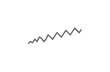
\begin{tikzpicture}[x=0.08em, y=0.08em, line width=0.4pt]
                \draw[FooterGray] (0,3) -- (1,4) -- (2,3.5) -- (3,5) -- (4,4) -- (5,6) -- (6,5.5) -- (7,4) -- (8,5) -- (9,7) -- (10,6) -- (11,5) -- (12,6.5) -- (13,8) -- (14,7) -- (15,6) -- (16,7.5) -- (17,9) -- (18,8) -- (19,7) -- (20,8.5) -- (21,10) -- (22,9) -- (23,8) -- (24,9.5);
            \end{tikzpicture}%
        }%
        \hskip0.5cm%
    }%
    \vskip6pt%
}

%=============================================================================
% PACHETE
%=============================================================================
\usepackage[utf8]{inputenc}
\usepackage[T1]{fontenc}
\usepackage[romanian]{babel}
\usepackage{amsmath, amssymb, amsthm}
\usepackage{mathtools}
\usepackage{bm}
\usepackage{tikz}
\usetikzlibrary{arrows.meta, positioning, shapes, calc, decorations.pathreplacing, shadings}
\usepackage{booktabs}
\usepackage{multirow}
\usepackage{array}
\usepackage{graphicx}
\usepackage{hyperref}
\usepackage{colortbl}
\hypersetup{colorlinks=true, linkcolor=MainBlue, urlcolor=MainBlue}
\graphicspath{{../../logos/}{../../charts/}}
\hfuzz=2pt  % Suppress tiny overfull warnings (<2pt)
\vfuzz=2pt  % Suppress tiny vertical overfull warnings (<2pt)

%=============================================================================
% COMANDA QUANTLET
%=============================================================================
\newcommand{\quantlet}[2]{%
    \hfill\href{#2}{%
        \raisebox{-0.15em}{\includegraphics[height=0.7em]{ql_logo.png}}%
        \textcolor{MainBlue}{\tiny\ #1}%
    }%
}

%=============================================================================
%=============================================================================
% CENTRED MINIPAGE (fara spatiu vertical suplimentar)
%=============================================================================
\newenvironment{cminipage}[1]{%
    \par\noindent\hfill\begin{minipage}{#1}\ignorespaces
}{%
    \end{minipage}\hfill\null\par
}


% COMENZI PERSONALIZATE
%=============================================================================
\newcommand{\E}{\mathbb{E}}
\newcommand{\Var}{\text{Var}}
\newcommand{\Cov}{\text{Cov}}
\newcommand{\Corr}{\text{Corr}}
\newcommand{\R}{\mathbb{R}}
\newcommand{\RMSE}{\text{RMSE}}
\newcommand{\MAE}{\text{MAE}}
\newcommand{\MAPE}{\text{MAPE}}

% Quiz styling
\newcommand{\correct}{\textcolor{Forest}{\checkmark}}
\newcommand{\incorrect}{\textcolor{Crimson}{\texttimes}}

%=============================================================================
% PAGINĂ TITLU PERSONALIZATĂ
%=============================================================================
\defbeamertemplate*{title page}{hybrid}[1][]
{
    \vspace{0.2cm}
    % Logos row - top header (with clickable links)
    \begin{center}
        \href{https://www.ase.ro}{\includegraphics[height=1.0cm]{ase_logo.png}}\hspace{0.3cm}%
        \href{https://theida.net}{\includegraphics[height=1.0cm]{ida_logo.png}}\hspace{0.3cm}%
        \href{https://blockchain-research-center.com}{\includegraphics[height=1.0cm]{brc_logo.png}}\hspace{0.3cm}%
        \href{https://www.ai4efin.ase.ro}{\includegraphics[height=1.0cm]{ai4efin_logo.png}}\hspace{0.3cm}%
        \href{https://ipe.ro/new}{\includegraphics[height=1.0cm]{acad_logo.png}}\hspace{0.3cm}%
        \href{https://www.digital-finance-msca.com}{\includegraphics[height=1.0cm]{msca_logo.png}}%
    \end{center}

    \vspace{0.6cm}

    % Main title with Q logos on sides (with clickable links)
    \begin{center}
        \begin{minipage}{0.1\textwidth}
            \centering
            \href{https://quantlet.com}{\includegraphics[height=1.1cm]{ql_logo.png}}
        \end{minipage}%
        \begin{minipage}{0.78\textwidth}
            \centering
            {\LARGE\bfseries\usebeamercolor[fg]{title}\inserttitle}

            \vspace{0.3cm}

            {\usebeamerfont{subtitle}\usebeamercolor[fg]{title}\insertsubtitle}
        \end{minipage}%
        \begin{minipage}{0.1\textwidth}
            \centering
            \href{https://quantinar.com}{\includegraphics[height=1.1cm]{qr_logo.png}}
        \end{minipage}
    \end{center}

    \vspace{0.6cm}

    % Authors (left aligned)
    \hspace{0.5cm}{\usebeamerfont{author}\insertauthor}

    \vspace{0.3cm}

    % Institute/Affiliations (left aligned)
    \hspace{0.5cm}\begin{minipage}[t]{0.9\textwidth}
        \raggedright\small\insertinstitute
    \end{minipage}
}

%=============================================================================
% TITLE INFORMATION
%=============================================================================
\title[Analiza Seriilor de Timp]{Analiza și Prognoza seriilor de timp}
\subtitle{Seminar 2: Modele ARMA}
\author[D.T. Pele]{Daniel Traian PELE}
\institute{Academia de Studii Economice din București\\
IDA Institute Digital Assets\\
Blockchain Research Center\\
AI4EFin Artificial Intelligence for Energy Finance\\
Academia Română, Institutul de Prognoză Economică\\
MSCA Digital Finance}
\date{}

\begin{document}

% Title page (no header/footer)
{
\setbeamertemplate{headline}{}
\setbeamertemplate{footline}{}
\begin{frame}
    \titlepage
\end{frame}
}

%=============================================================================
% SEMINAR OUTLINE
%=============================================================================
\section{Prezentare Generală}

\begin{frame}{Cuprins Seminar}
    \begin{cminipage}{0.95\textwidth}
    \textbf{\large Activitățile de Astăzi:}

    \vspace{0.4cm}

    \begin{enumerate}
        \item[\textcolor{MainBlue}{\textbf{1.}}] \textbf{Test de recapitulare} --- Verificarea înțelegerii conceptelor ARMA
        \vspace{0.15cm}
        \item[\textcolor{MainBlue}{\textbf{2.}}] \textbf{Întrebări Adevărat/Fals} --- Verificări conceptuale
        \vspace{0.15cm}
        \item[\textcolor{MainBlue}{\textbf{3.}}] \textbf{Probleme practice} --- Practică cu AR/MA
        \vspace{0.15cm}
        \item[\textcolor{MainBlue}{\textbf{4.}}] \textbf{Exemple rezolvate} --- Ajustare și diagnostice
        \vspace{0.15cm}
        \item[\textcolor{MainBlue}{\textbf{5.}}] \textbf{Subiecte de discuție} --- Aplicații practice
        \vspace{0.15cm}
        \item[\textcolor{MainBlue}{\textbf{6.}}] \textbf{Exerciții cu asistență AI} --- Modelare om vs.\ AI
    \end{enumerate}
    \end{cminipage}
\end{frame}

%=============================================================================
% PART 1: TEST DE RECAPITULARE
%=============================================================================
\section{Test de recapitulare}

\begin{frame}{Test 1: Operatorul Lag}
    \begin{cminipage}{0.95\textwidth}
    \begin{alertblock}{Întrebare}
        Care este rezultatul aplicării $(1-L)^2$ lui $X_t$?
    \end{alertblock}

    \vspace{0.5cm}
    \begin{block}{Variante de răspuns}
        \textcolor{MainBlue}{\textbf{(A)}} $X_t - X_{t-1}$ \qquad
{indent}    \textcolor{MainBlue}{\textbf{(B)}} $X_t - 2X_{t-1} + X_{t-2}$ \qquad
{indent}    \textcolor{MainBlue}{\textbf{(C)}} $X_t + X_{t-1} + X_{t-2}$ \qquad
{indent}    \textcolor{MainBlue}{\textbf{(D)}} $X_t - X_{t-2}$
    \end{block}
    \end{cminipage}
\end{frame}

\begin{frame}{Test 1: Răspuns}
    \begin{cminipage}{0.95\textwidth}
    \begin{columns}[T]
        \begin{column}{0.50\textwidth}
            \begin{exampleblock}{Răspuns: B}
                $X_t - 2X_{t-1} + X_{t-2}$
            \end{exampleblock}

            \vspace{0.2cm}

            \textbf{Explicație:}
            \begin{align*}
                (1-L)^2 X_t &= (1 - 2L + L^2)X_t \\
                &= X_t - 2X_{t-1} + X_{t-2}
            \end{align*}

            Aceasta este \textbf{diferența de ordinul doi} a lui $X_t$.
        \end{column}
        \begin{column}{0.48\textwidth}
            \includegraphics[width=\textwidth]{lag_operator.pdf}
            {\tiny Operatorul lag: $L^k X_t = X_{t-k}$}
        \end{column}
    \end{columns}
    
    \end{cminipage}
    \quantlet{TSA\_ch2\_lag\_operator}{https://github.com/QuantLet/TSA/tree/main/TSA_ch2/TSA_ch2_lag_operator}
\end{frame}

\begin{frame}{Test 2: Staționaritatea AR(1)}
    \begin{cminipage}{0.95\textwidth}
    \begin{alertblock}{Întrebare}
        Pentru ce valoare a lui $\phi$ procesul AR(1) $X_t = 0.5 + \phi X_{t-1} + \varepsilon_t$ este staționar?
    \end{alertblock}

    \vspace{0.5cm}
    \begin{block}{Variante de răspuns}
        \textcolor{MainBlue}{\textbf{(A)}} $\phi = 1.2$ \qquad
{indent}    \textcolor{MainBlue}{\textbf{(B)}} $\phi = 1.0$ \qquad
{indent}    \textcolor{MainBlue}{\textbf{(C)}} $\phi = -0.8$ \qquad
{indent}    \textcolor{MainBlue}{\textbf{(D)}} $\phi = -1.5$
    \end{block}
    \end{cminipage}
\end{frame}

\begin{frame}{Test 2: Răspuns}
    \begin{cminipage}{0.95\textwidth}
    \begin{columns}[T]
        \begin{column}{0.50\textwidth}
            \begin{exampleblock}{Răspuns: C}
                $\phi = -0.8$ (Staționar)
            \end{exampleblock}

            \vspace{0.2cm}

            \textbf{Condiția de staționaritate AR(1):}
            $$|\phi| < 1$$

            \vspace{0.2cm}

            Verificarea fiecărei opțiuni:
            \begin{itemize}
                \item A: $|1.2| = 1.2 > 1$ \incorrect
                \item B: $|1.0| = 1$ (rădăcină unitară) \incorrect
                \item C: $|-0.8| = 0.8 < 1$ \correct
                \item D: $|-1.5| = 1.5 > 1$ \incorrect
            \end{itemize}
        \end{column}
        \begin{column}{0.48\textwidth}
            \includegraphics[width=\textwidth]{ch2_def_ar1.pdf}
            {\tiny AR(1): regiunea staționară $|\phi| < 1$}
        \end{column}
    \end{columns}
    
    \end{cminipage}
    \quantlet{TSA\_ch2\_ar1}{https://github.com/QuantLet/TSA/tree/main/TSA_ch2/TSA_ch2_ar1}
\end{frame}

\begin{frame}{Test 3: Modelul ACF}
    \begin{cminipage}{0.95\textwidth}
    \begin{alertblock}{Întrebare}
        Observați următorul model ACF: vârf semnificativ la lag 1, apoi toate lag-urile în benzile de încredere. PACF arată descreștere graduală. Ce model este sugerat?
    \end{alertblock}

    \vspace{0.5cm}
    \begin{block}{Variante de răspuns}
        \textcolor{MainBlue}{\textbf{(A)}} AR(1) \qquad
{indent}    \textcolor{MainBlue}{\textbf{(B)}} MA(1) \qquad
{indent}    \textcolor{MainBlue}{\textbf{(C)}} ARMA(1,1) \qquad
{indent}    \textcolor{MainBlue}{\textbf{(D)}} Zgomot alb
    \end{block}
    \end{cminipage}
\end{frame}

\begin{frame}{Test 3: Răspuns}
    \begin{cminipage}{0.95\textwidth}
    \begin{columns}[T]
        \begin{column}{0.50\textwidth}
            \begin{exampleblock}{Răspuns: B}
                MA(1)
            \end{exampleblock}

            \vspace{0.2cm}

            \textbf{Regula cheie de identificare:}
            \begin{itemize}
                \item ACF se anulează după lag $q$ $\Rightarrow$ MA($q$)
                \item PACF se anulează după lag $p$ $\Rightarrow$ AR($p$)
            \end{itemize}

            \vspace{0.2cm}

            Aici: ACF se anulează la lag 1, PACF descrește

            $\Rightarrow$ \textbf{MA(1)}
        \end{column}
        \begin{column}{0.48\textwidth}
            \includegraphics[width=\textwidth]{ch2_def_ma1.pdf}
            {\tiny MA(1): ACF se anulează după lag 1}
        \end{column}
    \end{columns}
    
    \end{cminipage}
    \quantlet{TSA\_ch2\_ma1}{https://github.com/QuantLet/TSA/tree/main/TSA_ch2/TSA_ch2_ma1}
\end{frame}

\begin{frame}{Test 4: Invertibilitatea MA}
    \begin{cminipage}{0.95\textwidth}
    \begin{alertblock}{Întrebare}
        Pentru procesul MA(1) $X_t = \varepsilon_t + 1.5\varepsilon_{t-1}$, este procesul invertibil?
    \end{alertblock}

    \vspace{0.5cm}
    \begin{block}{Variante de răspuns}
        \textcolor{MainBlue}{\textbf{(A)}} Da, deoarece procesele MA sunt întotdeauna invertibile\\[3pt]
        \textcolor{MainBlue}{\textbf{(B)}} Da, deoarece $1.5 > 0$\\[3pt]
        \textcolor{MainBlue}{\textbf{(C)}} Nu, deoarece $|\theta| = 1.5 > 1$\\[3pt]
        \textcolor{MainBlue}{\textbf{(D)}} Nu, deoarece procesele MA nu sunt niciodată invertibile
    \end{block}
    \end{cminipage}
\end{frame}

\begin{frame}{Test 4: Răspuns}
    \begin{cminipage}{0.95\textwidth}
    \begin{columns}[T]
        \begin{column}{0.50\textwidth}
            \begin{exampleblock}{Răspuns: C}
                Nu este invertibil ($|\theta| = 1.5 > 1$)
            \end{exampleblock}

            \vspace{0.2cm}

            \textbf{Invertibilitatea MA(1):}

            Necesită $|\theta| < 1$

            \vspace{0.2cm}

            Echivalent: rădăcina lui $\theta(z) = 1 + \theta z = 0$ trebuie să fie în afara cercului unitate.

            Aici: $z = -1/1.5 = -0.67$ este \textbf{în interior}!

            \vspace{0.2cm}

            $\Rightarrow$ \textcolor{Crimson}{\textbf{Nu este invertibil}}
        \end{column}
        \begin{column}{0.48\textwidth}
            \includegraphics[width=\textwidth]{ch2_def_ma1.pdf}
            {\tiny Invertibilitate: rădăcina în afara cercului unitate}
        \end{column}
    \end{columns}
    
    \end{cminipage}
    \quantlet{TSA\_ch2\_ma1}{https://github.com/QuantLet/TSA/tree/main/TSA_ch2/TSA_ch2_ma1}
\end{frame}

\begin{frame}{Test 5: Reprezentarea ARMA}
    \begin{cminipage}{0.95\textwidth}
    \begin{alertblock}{Întrebare}
        Forma compactă $\phi(L)X_t = \theta(L)\varepsilon_t$ reprezintă ce model?
    \end{alertblock}

    \vspace{0.5cm}
    \begin{block}{Variante de răspuns}
        \textcolor{MainBlue}{\textbf{(A)}} Model AR pur\\[3pt]
        \textcolor{MainBlue}{\textbf{(B)}} Model MA pur\\[3pt]
        \textcolor{MainBlue}{\textbf{(C)}} Model ARMA\\[3pt]
        \textcolor{MainBlue}{\textbf{(D)}} Niciunul dintre cele de mai sus
    \end{block}
    \end{cminipage}
\end{frame}

\begin{frame}{Test 5: Răspuns}
    \begin{cminipage}{0.95\textwidth}
    \begin{columns}[T]
        \begin{column}{0.50\textwidth}
            \begin{exampleblock}{Răspuns: C}
                Model ARMA
            \end{exampleblock}

            \vspace{0.2cm}

            \textbf{Notația cu polinoame lag:}
            \begin{itemize}
                \item $\phi(L) = 1 - \phi_1 L - \cdots - \phi_p L^p$
                \item $\theta(L) = 1 + \theta_1 L + \cdots + \theta_q L^q$
            \end{itemize}

            \vspace{0.2cm}

            Cazuri speciale:
            \begin{itemize}
                \item $\theta(L) = 1$: AR pur
                \item $\phi(L) = 1$: MA pur
            \end{itemize}
        \end{column}
        \begin{column}{0.48\textwidth}
            \includegraphics[width=\textwidth]{ch2_def_arma.pdf}
            {\tiny ARMA(1,1): combină AR și MA}
        \end{column}
    \end{columns}
    
    \end{cminipage}
    \quantlet{TSA\_ch2\_arma}{https://github.com/QuantLet/TSA/tree/main/TSA_ch2/TSA_ch2_arma}
\end{frame}

\begin{frame}{Test 6: Criterii Informaționale}
    \begin{cminipage}{0.95\textwidth}
    \begin{alertblock}{Întrebare}
        Când comparăm ARMA(1,1) și ARMA(2,1) folosind BIC, care afirmație este corectă?
    \end{alertblock}

    \vspace{0.5cm}
    \begin{block}{Variante de răspuns}
        \textcolor{MainBlue}{\textbf{(A)}} BIC mai mic înseamnă întotdeauna prognoze mai bune\\[3pt]
        \textcolor{MainBlue}{\textbf{(B)}} BIC penalizează complexitatea mai puțin decât AIC\\[3pt]
        \textcolor{MainBlue}{\textbf{(C)}} Modelul cu BIC mai mic este preferat\\[3pt]
        \textcolor{MainBlue}{\textbf{(D)}} BIC poate compara doar modele cu același număr de parametri
    \end{block}
    \end{cminipage}
\end{frame}

\begin{frame}{Test 6: Răspuns}
    \begin{cminipage}{0.95\textwidth}
    \begin{columns}[T]
        \begin{column}{0.50\textwidth}
            \begin{exampleblock}{Răspuns: C}
                Modelul cu BIC mai mic este preferat
            \end{exampleblock}

            \vspace{0.2cm}

            \textbf{Criterii Informaționale:}
            \begin{align*}
                \text{AIC} &= -2\ln(\hat{L}) + 2k \\
                \text{BIC} &= -2\ln(\hat{L}) + k\ln(n)
            \end{align*}
            \vspace{-0.3cm}
            {\scriptsize $\hat{L}$ = maximul funcției de verosimilitate, $k$ = nr.\ parametri, $n$ = eșantion}

            \vspace{0.1cm}
            BIC penalizează complexitatea \textbf{mai mult} decât AIC (pentru $n > 7$).

            \vspace{0.2cm}

            $\Rightarrow$ BIC favorizează modele mai simple.
        \end{column}
        \begin{column}{0.48\textwidth}
            \includegraphics[width=\textwidth]{ch2_acf_pacf_patterns.pdf}
            {\tiny Selecția modelului: AIC vs BIC}
        \end{column}
    \end{columns}
    
    \end{cminipage}
    \quantlet{TSA\_ch2\_model\_selection}{https://github.com/QuantLet/TSA/tree/main/TSA_ch2/TSA_ch2_model_selection}
\end{frame}

\begin{frame}{Test 7: Testul Ljung-Box}
    \begin{cminipage}{0.95\textwidth}
    \begin{alertblock}{Întrebare}
        După ajustarea unui model ARMA(2,1), rulați testul Ljung-Box pe reziduuri și obțineți valoare-p = 0.02. Ce concluzie trageți?
    \end{alertblock}

    \vspace{0.5cm}
    \begin{block}{Variante de răspuns}
        \textcolor{MainBlue}{\textbf{(A)}} Modelul este adecvat\\[3pt]
        \textcolor{MainBlue}{\textbf{(B)}} Reziduurile sunt zgomot alb\\[3pt]
        \textcolor{MainBlue}{\textbf{(C)}} Există autocorelație semnificativă în reziduuri\\[3pt]
        \textcolor{MainBlue}{\textbf{(D)}} Modelul are prea mulți parametri
    \end{block}
    \end{cminipage}
\end{frame}

\begin{frame}{Test 7: Răspuns}
    \begin{cminipage}{0.95\textwidth}
    \begin{columns}[T]
        \begin{column}{0.50\textwidth}
            \begin{exampleblock}{Răspuns: C}
                Autocorelație semnificativă în reziduuri
            \end{exampleblock}

            \vspace{0.2cm}

            \textbf{Testul Ljung-Box:}
            \begin{itemize}
                \item $H_0$: Reziduurile sunt zgomot alb
                \item $H_1$: Autocorelație prezentă
            \end{itemize}

            \vspace{0.2cm}

            valoare-p = 0.02 $<$ 0.05

            $\Rightarrow$ \textcolor{Crimson}{\textbf{Respingem $H_0$}}

            Modelul este \textbf{inadecvat} --- încercați alte ordine.
        \end{column}
        \begin{column}{0.48\textwidth}
            \includegraphics[width=\textwidth]{ch2_diagnostics.pdf}
            {\tiny Diagnostice: ACF trebuie să fie zgomot alb}
        \end{column}
    \end{columns}
    
    \end{cminipage}
    \quantlet{TSA\_ch2\_diagnostics}{https://github.com/QuantLet/TSA/tree/main/TSA_ch2/TSA_ch2_diagnostics}
\end{frame}

\begin{frame}{Test 8: Prognoză}
    \begin{cminipage}{0.95\textwidth}
    \begin{alertblock}{Întrebare}
        Pentru un model AR(1) cu $\phi = 0.6$ și medie $\mu = 10$, ce se întâmplă cu prognozele când orizontul $h \to \infty$?
    \end{alertblock}

    \vspace{0.5cm}
    \begin{block}{Variante de răspuns}
        \textcolor{MainBlue}{\textbf{(A)}} Prognozele cresc fără limită\\[3pt]
        \textcolor{MainBlue}{\textbf{(B)}} Prognozele converg la 0\\[3pt]
        \textcolor{MainBlue}{\textbf{(C)}} Prognozele converg la $\mu = 10$\\[3pt]
        \textcolor{MainBlue}{\textbf{(D)}} Prognozele oscilează pentru totdeauna
    \end{block}
    \end{cminipage}
\end{frame}

\begin{frame}{Test 8: Răspuns}
    \begin{cminipage}{0.95\textwidth}
    \begin{columns}[T]
        \begin{column}{0.50\textwidth}
            \begin{exampleblock}{Răspuns: C}
                Prognozele converg la $\mu = 10$
            \end{exampleblock}

            \vspace{0.2cm}

            \textbf{Formula de prognoză AR(1):}
            $$\hat{X}_{n+h|n} = \mu + \phi^h(X_n - \mu)$$

            Deoarece $|\phi| = 0.6 < 1$:
            $$\lim_{h \to \infty} \phi^h = 0$$

            $\Rightarrow$ Prognozele converg la $\mu$.

            \textbf{Revenire la medie!}
        \end{column}
        \begin{column}{0.48\textwidth}
            \includegraphics[width=\textwidth]{ch2_ar1_forecast.pdf}
            {\tiny Prognoze AR(1): revenire la medie}
        \end{column}
    \end{columns}
    
    \end{cminipage}
    \quantlet{TSA\_ch2\_forecasting}{https://github.com/QuantLet/TSA/tree/main/TSA_ch2/TSA_ch2_forecasting}
\end{frame}

\begin{frame}{Test 9: Rădăcinile AR(2)}
    \begin{cminipage}{0.95\textwidth}
    \begin{alertblock}{Întrebare}
        Un proces AR(2) are rădăcinile caracteristice $z_1 = 0.8$ și $z_2 = -0.5$. Este staționar?
    \end{alertblock}

    \vspace{0.5cm}
    \begin{block}{Variante de răspuns}
        \textcolor{MainBlue}{\textbf{(A)}} Da, deoarece ambele rădăcini sunt în interiorul cercului unitate\\[3pt]
        \textcolor{MainBlue}{\textbf{(B)}} Nu, deoarece o rădăcină este negativă\\[3pt]
        \textcolor{MainBlue}{\textbf{(C)}} Nu, deoarece rădăcinile trebuie să fie în afara cercului unitate\\[3pt]
        \textcolor{MainBlue}{\textbf{(D)}} Nu se poate determina fără mai multe informații
    \end{block}
    \end{cminipage}
\end{frame}

\begin{frame}{Test 9: Răspuns}
    \begin{cminipage}{0.95\textwidth}
    \begin{columns}[T]
        \begin{column}{0.50\textwidth}
            \begin{exampleblock}{Răspuns: C}
                Rădăcinile trebuie să fie în afara cercului unitate
            \end{exampleblock}

            \vspace{0.2cm}

            \textbf{Condiția de staționaritate:}

            Rădăcinile lui $\phi(z) = 0$ trebuie să fie \textbf{în afara} cercului unitate ($|z| > 1$).

            \vspace{0.2cm}

            Aici:
            \begin{itemize}
                \item $|z_1| = 0.8 < 1$ \incorrect
                \item $|z_2| = 0.5 < 1$ \incorrect
            \end{itemize}

            Ambele în interior $\Rightarrow$ \textcolor{Crimson}{\textbf{Nestaționar}}
        \end{column}
        \begin{column}{0.48\textwidth}
            \includegraphics[width=\textwidth]{ch2_ar2_stationarity.pdf}
            {\tiny AR(2): rădăcini și triunghiul de staționaritate}
        \end{column}
    \end{columns}
    
    \end{cminipage}
    \quantlet{TSA\_ch2\_ar2}{https://github.com/QuantLet/TSA/tree/main/TSA_ch2/TSA_ch2_ar2}
\end{frame}

\begin{frame}{Test 10: Proprietățile MA(q)}
    \begin{cminipage}{0.95\textwidth}
    \begin{alertblock}{Întrebare}
        Pentru un proces MA(2), ACF-ul:
    \end{alertblock}

    \vspace{0.5cm}
    \begin{block}{Variante de răspuns}
        \textcolor{MainBlue}{\textbf{(A)}} Descrește exponențial \qquad
{indent}    \textcolor{MainBlue}{\textbf{(B)}} Se anulează după lag 2 \qquad
{indent}    \textcolor{MainBlue}{\textbf{(C)}} Se anulează după lag 1 \qquad
{indent}    \textcolor{MainBlue}{\textbf{(D)}} Nu se anulează niciodată
    \end{block}
    \end{cminipage}
\end{frame}

\begin{frame}{Test 10: Răspuns}
    \begin{cminipage}{0.95\textwidth}
    \begin{columns}[T]
        \begin{column}{0.50\textwidth}
            \begin{exampleblock}{Răspuns: B}
                Se anulează după lag 2
            \end{exampleblock}

            \vspace{0.2cm}

            \textbf{Proprietatea ACF pentru MA($q$):}

            $$\rho(h) = 0 \text{ pentru } h > q$$

            \vspace{0.2cm}

            \begin{itemize}
                \item MA(1): ACF se anulează după lag 1
                \item MA(2): ACF se anulează după lag 2
                \item MA($q$): ACF se anulează după lag $q$
            \end{itemize}

            Caracteristica cheie de identificare!
        \end{column}
        \begin{column}{0.48\textwidth}
            \includegraphics[width=\textwidth]{ch2_def_ma1.pdf}
            {\tiny MA: anularea ACF este semnătura}
        \end{column}
    \end{columns}
    
    \end{cminipage}
    \quantlet{TSA\_ch2\_ma1}{https://github.com/QuantLet/TSA/tree/main/TSA_ch2/TSA_ch2_ma1}
\end{frame}

%=============================================================================
% PART 2: TRUE/FALSE QUESTIONS
%=============================================================================
\section{Întrebări Adevărat/Fals}

\begin{frame}{Adevărat sau Fals? --- Întrebări}
    \begin{cminipage}{0.95\textwidth}
    \footnotesize
    \begin{center}
    \begin{tabular}{p{9cm}c}
        \toprule
        \textbf{Afirmație} & \textbf{A/F?} \\
        \midrule
        1. Un proces AR(2) poate prezenta comportament pseudo-ciclic. & ? \\[0.15cm]
        2. Procesele MA necesită o condiție de staționaritate. & ? \\[0.15cm]
        3. PACF-ul unui proces AR(p) se anulează după lag $p$. & ? \\[0.15cm]
        4. Dacă AIC selectează ARMA(2,1) și BIC selectează ARMA(1,1), nu pot fi ambele corecte. & ? \\[0.15cm]
        5. Intervalele de încredere se îngustează pe măsură ce orizontul crește. & ? \\[0.15cm]
        6. Ecuațiile Yule-Walker pot fi folosite pentru a estima parametrii MA. & ? \\
        \bottomrule
    \end{tabular}
    \end{center}
    \end{cminipage}
\end{frame}

\begin{frame}{Adevărat sau Fals? --- Răspunsuri}
    \begin{cminipage}{0.95\textwidth}
    \begin{columns}[T]
        \begin{column}{0.52\textwidth}
            \small
            \begin{enumerate}
                \item \textcolor{Forest}{\textbf{ADEVĂRAT}}: AR(2) cu rădăcini complexe $\Rightarrow$ oscilații amortizate
                \vspace{0.1cm}
                \item \textcolor{Crimson}{\textbf{FALS}}: Procesele MA sunt întotdeauna staționare; au nevoie de \textit{invertibilitate}
                \vspace{0.1cm}
                \item \textcolor{Forest}{\textbf{ADEVĂRAT}}: Caracteristica cheie de identificare a AR($p$)
                \vspace{0.1cm}
                \item \textcolor{Crimson}{\textbf{FALS}}: Ambele sunt „corecte" pentru criteriile lor (AIC: estimare, BIC: parsimonie)
                \vspace{0.1cm}
                \item \textcolor{Crimson}{\textbf{FALS}}: IC se \textit{lărgesc} cu orizontul (mai multă incertitudine)
                \vspace{0.1cm}
                \item \textcolor{Crimson}{\textbf{FALS}}: Yule-Walker este pentru AR; MA folosește MLE
            \end{enumerate}
        \end{column}
        \begin{column}{0.46\textwidth}
            \includegraphics[width=\textwidth]{ch2_ar2_stationarity.pdf}
            {\tiny AR(2): rădăcini complexe $\Rightarrow$ cicluri}
        \end{column}
    \end{columns}
    
    \end{cminipage}
    \quantlet{TSA\_ch2\_ar2}{https://github.com/QuantLet/TSA/tree/main/TSA_ch2/TSA_ch2_ar2}
\end{frame}

%=============================================================================
% PART 3: PROBLEME PRACTICE
%=============================================================================
\section{Probleme practice}

\begin{frame}{Exercițiul 1: Proprietățile AR(1)}
    \begin{cminipage}{0.95\textwidth}
    \textbf{Problemă:} Considerați procesul AR(1):
    $$X_t = 2 + 0.7 X_{t-1} + \varepsilon_t, \quad \varepsilon_t \sim WN(0, 9)$$

    Calculați:
    \begin{enumerate}
        \item Media $\mu$
        \item Varianța $\gamma(0)$
        \item Autocovarianța $\gamma(1)$ și $\gamma(2)$
        \item Autocorelația $\rho(1)$ și $\rho(2)$
    \end{enumerate}
    \end{cminipage}
\end{frame}

\begin{frame}{Exercițiul 1: Soluție}
    \begin{cminipage}{0.95\textwidth}
    \small
    \begin{columns}[T]
        \begin{column}{0.55\textwidth}
            Dat: $c = 2$, $\phi = 0.7$, $\sigma^2 = 9$

            \vspace{0.1cm}
            \textbf{1. Media:}
            $\mu = \frac{c}{1-\phi} = \frac{2}{1-0.7} = \frac{2}{0.3} = \textbf{6.67}$

            \textbf{2. Varianța:}
            $\gamma(0) = \frac{\sigma^2}{1-\phi^2} = \frac{9}{1-0.49} = \textbf{17.65}$

            \textbf{3. Autocovarianța:}
            $\gamma(1) = \phi \cdot \gamma(0) = 0.7 \times 17.65 = \textbf{12.35}$\\
            $\gamma(2) = \phi^2 \cdot \gamma(0) = 0.49 \times 17.65 = \textbf{8.65}$

            \textbf{4. Autocorelația:}
            $\rho(1) = \phi = \textbf{0.7}, \quad \rho(2) = \phi^2 = \textbf{0.49}$
        \end{column}
        \begin{column}{0.43\textwidth}
            \includegraphics[width=\textwidth]{ch2_ar1_simulations.pdf}
            {\tiny Simulare AR(1) și ACF}
        \end{column}
    \end{columns}
    
    \end{cminipage}
    \quantlet{TSA\_ch2\_ex1\_ar1}{https://github.com/QuantLet/TSA/tree/main/TSA_ch2/TSA_ch2_ex1_ar1}
\end{frame}

\begin{frame}{Exercițiul 2: Proprietățile MA(1)}
    \begin{cminipage}{0.95\textwidth}
    \textbf{Problemă:} Considerați procesul MA(1):
    $$X_t = 5 + \varepsilon_t - 0.4\varepsilon_{t-1}, \quad \varepsilon_t \sim WN(0, 4)$$

    Calculați:
    \begin{enumerate}
        \item Media $\mu$
        \item Varianța $\gamma(0)$
        \item Autocovarianța $\gamma(1)$
        \item Autocorelația $\rho(1)$
        \item Este acest proces invertibil?
    \end{enumerate}
    \end{cminipage}
\end{frame}

\begin{frame}{Exercițiul 2: Soluție}
    \begin{cminipage}{0.95\textwidth}
    \small
    \begin{columns}[T]
        \begin{column}{0.55\textwidth}
            Dat: $\mu = 5$, $\theta = -0.4$, $\sigma^2 = 4$

            \vspace{0.1cm}
            \textbf{1. Media:} $\E[X_t] = \mu = \textbf{5}$

            \textbf{2. Varianța:} $\gamma(0) = \sigma^2(1 + \theta^2) = 4(1.16) = \textbf{4.64}$

            \textbf{3. Autocovarianța:} $\gamma(1) = \theta\sigma^2 = -0.4 \times 4 = \textbf{-1.6}$

            \textbf{4. Autocorelația:} $\rho(1) = \frac{\gamma(1)}{\gamma(0)} = \frac{-1.6}{4.64} = \textbf{-0.345}$

            \textbf{5. Invertibilitate:} $|\theta| = 0.4 < 1$ $\Rightarrow$ \textcolor{Forest}{\textbf{Da}}
        \end{column}
        \begin{column}{0.43\textwidth}
            \includegraphics[width=\textwidth]{ch2_ma1_simulations.pdf}
            {\tiny MA(1): ACF se anulează după lag 1}
        \end{column}
    \end{columns}
    
    \end{cminipage}
    \quantlet{TSA\_ch2\_ex2\_ma1}{https://github.com/QuantLet/TSA/tree/main/TSA_ch2/TSA_ch2_ex2_ma1}
\end{frame}

\begin{frame}{Exercițiul 3: Rădăcinile Caracteristice}
    \begin{cminipage}{0.95\textwidth}
    \textbf{Problemă:} Considerați procesul AR(2):
    $$X_t = 0.5X_{t-1} + 0.3X_{t-2} + \varepsilon_t$$

    \begin{enumerate}
        \item Scrieți ecuația caracteristică
        \item Găsiți rădăcinile caracteristice
        \item Este acest proces staționar?
    \end{enumerate}
    \end{cminipage}
\end{frame}

\begin{frame}{Exercițiul 3: Soluție}
    \begin{cminipage}{0.95\textwidth}
    \begin{columns}[T]
        \begin{column}{0.55\textwidth}
            \textbf{1. Ecuația caracteristică:}
            $$\phi(z) = 1 - 0.5z - 0.3z^2 = 0$$
            Sau: $0.3z^2 + 0.5z - 1 = 0$

            \vspace{0.2cm}
            \textbf{2. Rădăcinile (formula cuadratică):}
            $$z = \frac{-0.5 \pm \sqrt{0.25 + 1.2}}{0.6}$$
            $$z_1 = \textbf{1.17}, \quad z_2 = \textbf{-2.84}$$

            \vspace{0.2cm}
            \textbf{3. Verificarea staționarității:}

            $|z_1| = 1.17 > 1$ \correct

            $|z_2| = 2.84 > 1$ \correct

            Ambele în afara cercului unitate $\Rightarrow$ \textcolor{Forest}{\textbf{Staționar}}
        \end{column}
        \begin{column}{0.43\textwidth}
            \includegraphics[width=\textwidth]{ch2_ar2_stationarity.pdf}
            {\tiny Rădăcini în afara cercului $\Rightarrow$ staționar}
        \end{column}
    \end{columns}
    
    \end{cminipage}
    \quantlet{TSA\_ch2\_ex3\_roots}{https://github.com/QuantLet/TSA/tree/main/TSA_ch2/TSA_ch2_ex3_roots}
\end{frame}

\begin{frame}{Exercițiul 4: Prognoză}
    \begin{cminipage}{0.95\textwidth}
    \textbf{Problemă:} Ați ajustat un model AR(1):
    $$X_t = 3 + 0.8X_{t-1} + \varepsilon_t, \quad \sigma^2 = 4$$

    Dat $X_{100} = 20$, calculați:
    \begin{enumerate}
        \item Prognoza la 1 pas înainte $\hat{X}_{101|100}$
        \item Prognoza la 2 pași înainte $\hat{X}_{102|100}$
        \item Prognoza pe termen lung când $h \to \infty$
        \item Intervalul de încredere de 95\% pentru $\hat{X}_{101|100}$
    \end{enumerate}
    \end{cminipage}
\end{frame}

\begin{frame}{Exercițiul 4: Soluție}
    \begin{cminipage}{0.95\textwidth}
    \begin{columns}[T]
        \begin{column}{0.55\textwidth}
            Dat: $c = 3$, $\phi = 0.8$, $\sigma^2 = 4$, $X_{100} = 20$

            \textbf{Media:} $\mu = \frac{3}{1-0.8} = \textbf{15}$

            \vspace{0.1cm}
            \textbf{1. Prognoza la un pas:}
            $\hat{X}_{101|100} = 3 + 0.8 \times 20 = \textbf{19}$

            \textbf{2. Prognoza la doi pași:}
            $\hat{X}_{102|100} = 3 + 0.8 \times 19 = \textbf{18.2}$

            \textbf{3. Prognoza pe termen lung:}
            $\lim_{h \to \infty} \hat{X}_{100+h|100} = \mu = \textbf{15}$

            \textbf{4. IC 95\%:}
            $19 \pm 1.96 \times 2 = \textbf{[15.08, 22.92]}$
        \end{column}
        \begin{column}{0.43\textwidth}
            \includegraphics[width=\textwidth]{ch2_ar1_forecast.pdf}
            {\tiny Prognoza converge la medie}
        \end{column}
    \end{columns}
    
    \end{cminipage}
    \quantlet{TSA\_ch2\_ex4\_forecast}{https://github.com/QuantLet/TSA/tree/main/TSA_ch2/TSA_ch2_ex4_forecast}
\end{frame}

%=============================================================================
% PART 4: EXEMPLE REZOLVATE
%=============================================================================
\section{Exemple rezolvate}

\begin{frame}[fragile]{Exercițiu Python 1: Simulare și Ajustare AR(1)}
    \textbf{Sarcină:}
    \begin{enumerate}
        \item Simulați 300 de observații dintr-un AR(1) cu $\phi = 0.6$
        \item Reprezentați grafic seria și ACF/PACF
        \item Ajustați un model AR(1) și comparați $\hat{\phi}$ vs $\phi$ real
        \item Examinați diagnosticele reziduurilor
    \end{enumerate}

    \vspace{0.3cm}
    \textbf{Cod cheie:}
    \begin{verbatim}
from statsmodels.tsa.arima.model import ARIMA
model = ARIMA(x, order=(1, 0, 0)).fit()
print(model.summary())
    \end{verbatim}

    \quantlet{TSA\_ch2\_python\_simulate}{https://github.com/QuantLet/TSA/tree/main/TSA_ch2/TSA_ch2_python_simulate}
\end{frame}

\begin{frame}{Exercițiu Python 2: Selecția modelului}
    \begin{cminipage}{0.95\textwidth}
    \textbf{Sarcină:}
    \begin{enumerate}
        \item Încărcați o serie de timp și verificați staționaritatea (testul ADF)
        \item Comparați AIC/BIC pentru AR(1), MA(1), ARMA(1,1), ARMA(2,1)
        \item Selectați cel mai bun model
        \item Generați prognoze cu intervale de încredere
    \end{enumerate}

    \vspace{0.3cm}
    \textbf{Funcții cheie:}
    \begin{itemize}
        \item \texttt{adfuller(x)} pentru testul de staționaritate
        \item \texttt{model.aic}, \texttt{model.bic} pentru criterii
        \item \texttt{model.get\_forecast(h)} pentru predicții
    \end{itemize}

    
    \end{cminipage}
    \quantlet{TSA\_ch2\_python\_selection}{https://github.com/QuantLet/TSA/tree/main/TSA_ch2/TSA_ch2_python_selection}
\end{frame}

\begin{frame}{Exercițiu Python 3: Verificarea Diagnosticelor}
    \begin{cminipage}{0.95\textwidth}
    \textbf{Sarcină:} După ajustarea unui model, efectuați diagnostice complete:
    \begin{enumerate}
        \item Reprezentați grafic reziduurile în timp
        \item Reprezentați grafic ACF-ul reziduurilor
        \item Creați graficul Q-Q pentru normalitate
        \item Rulați testul Ljung-Box
    \end{enumerate}

    \vspace{0.3cm}
    \textbf{Funcții cheie:}
    \begin{itemize}
        \item \texttt{model.resid} pentru reziduuri
        \item \texttt{plot\_acf(resid)} pentru graficul ACF
        \item \texttt{stats.probplot(resid)} pentru graficul Q-Q
        \item \texttt{acorr\_ljungbox(resid, lags=[10])} pentru test
    \end{itemize}

    
    \end{cminipage}
    \quantlet{TSA\_ch2\_python\_diagnostics}{https://github.com/QuantLet/TSA/tree/main/TSA_ch2/TSA_ch2_python_diagnostics}
\end{frame}

%=============================================================================
% PART 5: SUBIECTE DE DISCUȚIE
%=============================================================================
\section{Subiecte de discuție}

\begin{frame}{Discuție 1: Selecția modelului}
    \begin{cminipage}{0.95\textwidth}
    \textbf{Scenariu:} Modelați rate de inflație lunare. După verificarea staționarității:
    \begin{itemize}
        \item ACF: semnificativ la lag-urile 1, 2, 3, apoi descrește
        \item PACF: semnificativ la lag-urile 1, 2, apoi se anulează
        \item AIC selectează ARMA(2,3)
        \item BIC selectează AR(2)
    \end{itemize}

    \vspace{0.3cm}
    \textbf{Întrebări:}
    \begin{enumerate}
        \item Ce sugerează modelul ACF/PACF?
        \item De ce nu sunt de acord AIC și BIC?
        \item Ce model ați alege și de ce?
        \item Ce verificări suplimentare ați efectua?
    \end{enumerate}
    \end{cminipage}
\end{frame}

\begin{frame}{Discuție 2: Evaluarea prognozei}
    \begin{cminipage}{0.95\textwidth}
    \textbf{Scenariu:} Ajustați un model ARMA(1,1) pe randamente zilnice de acțiuni. Ajustarea în eșantion arată bine (Ljung-Box p = 0.45), dar RMSE în afara eșantionului este mai rău decât mersul aleatoriu.

    \vspace{0.3cm}
    \textbf{Întrebări:}
    \begin{enumerate}
        \item Este aceasta surprinzător? De ce sau de ce nu?
        \item Ce ne spune despre predictibilitatea randamentelor?
        \item Ar trebui să concluzionați că modelul ARMA este inutil?
        \item Ce alternative ați putea considera?
    \end{enumerate}

    \vspace{0.3cm}
    \textbf{Indiciu:} Gândiți-vă la Ipoteza Pieței Eficiente și la ce captează ARMA vs. volatility clustering.
    \end{cminipage}
\end{frame}

%=============================================================================
% EXERCIȚII CU ASISTENȚĂ AI
%=============================================================================
\section{Exerciții cu asistență AI}

\begin{frame}{AI în Modelarea ARMA}
    \begin{cminipage}{0.95\textwidth}
    \begin{block}{Context}
        {\small
        Instrumentele AI pot ajusta modele ARMA și genera diagnostice automat.
        Competența critică este \textbf{evaluarea corectitudinii metodologiei}.
        }
    \end{block}

    \vspace{0.3cm}

    \textbf{Întrebări cheie pentru orice analiză ARMA generată de AI:}
    \begin{enumerate}
        \item A verificat staționaritatea \textbf{înainte} de ajustare?
        \item Ordinul modelului este justificat de ACF/PACF?
        \item Reziduurile sunt zgomot alb (testul Ljung-Box)?
        \item Rădăcinile sunt în interiorul cercului unitate?
        \item Orizontul de prognoză este rezonabil pentru model?
    \end{enumerate}
    \end{cminipage}
\end{frame}

\begin{frame}{Exercițiu AI 1: Criticați o analiză AI}
    \begin{cminipage}{0.95\textwidth}
    \begin{block}{Scenariu}
        Ați cerut unui AI: „Ajustează cel mai bun model pe datele de pete solare." A returnat:
        \begin{itemize}
            \item A ajustat ARMA(4,3) cu AIC = 2415.3
            \item Niciun test de staționaritate efectuat
            \item Ljung-Box valoare-p = 0.03 (raportat ca „acceptabil")
            \item Prognoză pe 50 de ani cu intervale de încredere înguste
        \end{itemize}
    \end{block}

    \vspace{0.3cm}

    \textbf{Critica voastră:}
    \begin{enumerate}
        \item ARMA(4,3) este supra-parametrizat? Ce ar sugera BIC?
        \item De ce Ljung-Box p = 0.03 \textbf{nu} este acceptabil la pragul de 5\%?
        \item Prognozele pe 50 de ani sunt fiabile pentru modele ARMA? De ce?
        \item Care este metodologia Box-Jenkins corectă care a fost omisă?
    \end{enumerate}
    \end{cminipage}
\end{frame}

\begin{frame}{Exercițiu AI 2: Prompt Refinement pentru ARMA}
    \begin{cminipage}{0.95\textwidth}
    \begin{block}{Sarcina}
        Îmbunătățiți iterativ prompt-urile pentru ajustarea unui model AR pe datele de pete solare.
    \end{block}

    \vspace{0.2cm}

    \textbf{Runda 1} (vag): \textit{„Ajustează un model de serie de timp pe pete solare"}
    \begin{itemize}
        \item Ce a produs AI-ul? Ce lipsește?
    \end{itemize}

    \textbf{Runda 2} (mai bun): \textit{„Testează staționaritatea cu ADF, examinează ACF/PACF, ajustează AR(p) folosind BIC, verifică reziduurile cu Ljung-Box"}
    \begin{itemize}
        \item AI-ul a urmat metodologia Box-Jenkins?
    \end{itemize}

    \textbf{Runda 3} (expert): \textit{„Urmează Box-Jenkins: (1) trasează și testează staționaritatea, (2) identifică ordinul din ACF/PACF, (3) estimează AR(2), (4) Ljung-Box pe reziduuri, (5) prognozează 20 pași cu IC 95\%"}
    \begin{itemize}
        \item Comparați rezultatele din toate cele trei runde
    \end{itemize}
    \end{cminipage}
\end{frame}

\begin{frame}{Exercițiu AI 3: Competiție de selecție a modelului}
    \begin{cminipage}{0.95\textwidth}
    \begin{block}{Sarcina}
        Descărcați date lunare de șomaj din \texttt{statsmodels.datasets}.
    \end{block}

    \vspace{0.2cm}

    \textbf{Abordarea voastră (manuală):}
    \begin{itemize}
        \item Analiza ACF/PACF $\to$ modele candidate
        \item Comparați AIC/BIC pentru AR(1), AR(2), MA(1), ARMA(1,1)
        \item Diagnostice reziduale pentru modelul selectat
        \item Prognoză rolling pe ultimele 20 de observații
    \end{itemize}

    \vspace{0.2cm}

    \textbf{Abordare AI:}
    \begin{itemize}
        \item Cereți AI-ului să „găsească cel mai bun model ARMA și să prognozeze"
    \end{itemize}

    \vspace{0.2cm}

    \textbf{Comparați:}
    \begin{itemize}
        \item Ce model a selectat fiecare? Coincid?
        \item Comparați RMSE out-of-sample
        \item AI-ul a folosit prognoze rolling sau doar multi-step?
        \item \textbf{Predați:} reflecție de 1 pagină despre punctele forte și slabe ale AI
    \end{itemize}
    \end{cminipage}
\end{frame}

%=============================================================================
% KEY FORMULAS SUMMARY
%=============================================================================
\section{Formule cheie}

\begin{frame}{Rezumat Formule cheie}
    \begin{cminipage}{0.95\textwidth}
    \small
    \begin{center}
    \begin{tabular}{ll}
        \toprule
        \textbf{Concept} & \textbf{Formula} \\
        \midrule
        Media AR(1) & $\mu = c/(1-\phi)$ \\[0.1cm]
        Varianța AR(1) & $\gamma(0) = \sigma^2/(1-\phi^2)$ \\[0.1cm]
        ACF AR(1) & $\rho(h) = \phi^h$ \\[0.1cm]
        Staționaritate AR(1) & $|\phi| < 1$ \\[0.1cm]
        \midrule
        Varianța MA(1) & $\gamma(0) = \sigma^2(1+\theta^2)$ \\[0.1cm]
        ACF MA(1) & $\rho(1) = \theta/(1+\theta^2)$, $\rho(h) = 0$ pentru $h > 1$ \\[0.1cm]
        Invertibilitate MA(1) & $|\theta| < 1$ \\[0.1cm]
        \midrule
        Prognoza AR(1) & $\hat{X}_{n+h|n} = \mu + \phi^h(X_n - \mu)$ \\[0.1cm]
        IC Prognoză & $\hat{X} \pm z_{\alpha/2} \times \sqrt{\text{MSFE}(h)}$ \\[0.1cm]
        \midrule
        AIC & $-2\ln(\hat{L}) + 2k$ \\[0.1cm]
        BIC & $-2\ln(\hat{L}) + k\ln(n)$ \\
        \bottomrule
    \end{tabular}
    \end{center}
    \vspace{-0.1cm}
    {\scriptsize \textbf{Notații:} $\hat{L}$ = maximul funcției de verosimilitate, $k$ = nr.\ parametri, $n$ = dimensiunea eșantionului, $c$ = constantă, $\sigma^2$ = varianța zgomotului alb}
    \end{cminipage}
\end{frame}

%=============================================================================
% END
%=============================================================================
\begin{frame}
    \begin{cminipage}{0.95\textwidth}
    \centering
    \vspace{2cm}
    {\Huge\textcolor{MainBlue}{Întrebări?}}

    \vspace{1cm}

    \normalsize
    Succes la exerciții!

    \vspace{0.5cm}

    \textbf{Următorul Seminar:} ARIMA și Modele Sezoniere
    \end{cminipage}
\end{frame}


%=============================================================================
% BIBLIOGRAFIE
%=============================================================================
\begin{frame}{Bibliografie I}
    \begin{cminipage}{0.95\textwidth}
    \begin{block}{Manuale fundamentale}
        {\small
        \begin{itemize}
            \item Hyndman, R.J., \& Athanasopoulos, G. (2021). \textit{Forecasting: Principles and Practice}, 3rd ed., OTexts.
            \item Shumway, R.H., \& Stoffer, D.S. (2017). \textit{Time Series Analysis and Its Applications}, 4th ed., Springer.
            \item Brockwell, P.J., \& Davis, R.A. (2016). \textit{Introduction to Time Series and Forecasting}, 3rd ed., Springer.
        \end{itemize}
        }
    \end{block}

    \begin{exampleblock}{Serii de timp financiare}
        {\small
        \begin{itemize}
            \item Tsay, R.S. (2010). \textit{Analysis of Financial Time Series}, 3rd ed., Wiley.
            \item Franke, J., Härdle, W.K., \& Hafner, C.M. (2019). \textit{Statistics of Financial Markets}, 4th ed., Springer.
        \end{itemize}
        }
    \end{exampleblock}
    \end{cminipage}
\end{frame}

\begin{frame}{Bibliografie II}
    \begin{cminipage}{0.95\textwidth}
    \begin{block}{Abordari moderne si Machine Learning}
        {\small
        \begin{itemize}
            \item Nielsen, A. (2019). \textit{Practical Time Series Analysis}, O'Reilly Media.
            \item Petropoulos, F., et al. (2022). \textit{Forecasting: Theory and Practice}, International Journal of Forecasting.
            \item Makridakis, S., Spiliotis, E., \& Assimakopoulos, V. (2020). The M4 Competition, International Journal of Forecasting.
        \end{itemize}
        }
    \end{block}

    \begin{exampleblock}{Resurse online si cod}
        {\small
        \begin{itemize}
            \item \textbf{Quantlet}: \url{https://quantlet.com} --- Repository de cod pentru statistica
            \item \textbf{Quantinar}: \url{https://quantinar.com} --- Platforma de invatare metode cantitative
            \item \textbf{GitHub TSA}: \url{https://github.com/QuantLet/TSA/tree/main/TSA_ch2} --- Cod Python pentru acest seminar
        \end{itemize}
        }
    \end{exampleblock}
    \end{cminipage}
\end{frame}

\end{document}
